\begin{exo}
	On interroge au hasard $200$ personnes à la sortie d'une salle de cinéma à propos du roman dont le film qu'ils ont vu est une adaptation.

	$95$ personnes avaient lu le roman avant de venir voir le film et $140$ personnes ont aimé le film.

	De plus, parmi les personnes qui ont lu le roman, $55$ ont apprécié l'adaptation.

	On considère les événements :
	\begin{itemize}[label=$\bullet$]
		\item $F$ : \og{} la personne a aimé le film \fg{}
		\item $R$ : \og{} la personne a lu le roman \fg{}
	\end{itemize}

	\begin{enumerate}
		\item Reproduire et compléter le diagramme ci-contre.
	\end{enumerate}
	\begin{center}
		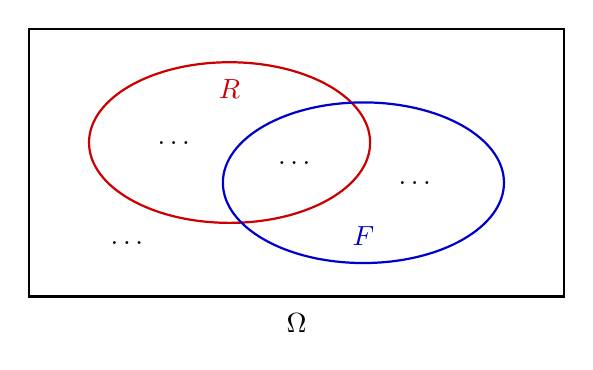
\begin{tikzpicture}[scale=0.85]
			\draw[thick] (0,0) rectangle (8,4);
			\node at (4,-0.4) {$\Omega$};

			\draw[red!80!black, thick] (3,2.3) ellipse (2.1 and 1.2);
			\node[red!80!black] at (3,3.1) {$R$};
			\node at (2.2,2.3) {\dots};

			\draw[blue!80!black, thick] (5,1.7) ellipse (2.1 and 1.2);
			\node[blue!80!black] at (5,0.9) {$F$};
			\node at (5.8,1.7) {\dots};

			\node at (4,2) {\dots};
			\node at (1.5,0.8) {\dots};
		\end{tikzpicture}
	\end{center}
	\begin{enumerate}[resume]
		\item Quelle est la probabilité qu'une personne n'ait pas aimé le film et n'ait pas lu le livre ?
		\item Définir par une phrase l'événement $R \cap \overline{F}$ et donner sa probabilité.
		\item Définir par une phrase l'événement $\overline{R} \cap F$ et donner sa probabilité.
	\end{enumerate}
\end{exo}
